%%% Appendix
\chapter{附录 代码与运行结果汇总}

\section{实验0. 通过键盘输入和文件输入}

\lstinputlisting[
        language = Java,
        caption = {\bf Problem0.java}    
]{../../../ProblemSet/src/Problem0.java}

\begin{figure}[H]
    \centering
    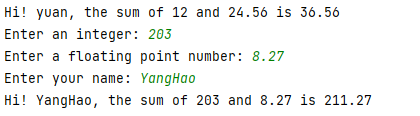
\includegraphics[width = 0.5\textwidth]{../pic/0.png}
    \caption{实验0运行结果}
\end{figure}

\newpage
\section{实验1. UPC码}

\lstinputlisting[
        language = Java,
        caption = {\bf Problem1.java}    
]{../../../ProblemSet/src/Problem1.java}

\begin{figure}[H]
	\centering
	\begin{subfigure}{0.325\linewidth}
		\centering
		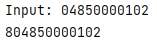
\includegraphics[width=0.7\linewidth]{../pic/1/1.1.png}
	\end{subfigure}
	\begin{subfigure}{0.325\linewidth}
		\centering
		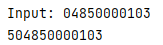
\includegraphics[width=0.7\linewidth]{../pic/1/1.2.png}
	\end{subfigure}
	\begin{subfigure}{0.325\linewidth}
		\centering
		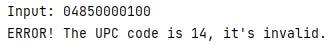
\includegraphics[width=1\linewidth]{../pic/1/1.3.png}
	\end{subfigure}
    \vspace{1cm}
    \begin{subfigure}{0.325\linewidth}
		\centering
		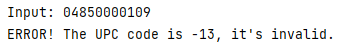
\includegraphics[width=1\linewidth]{../pic/1/1.4.png}
	\end{subfigure}
	\begin{subfigure}{0.325\linewidth}
		\centering
		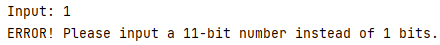
\includegraphics[width=1\linewidth]{../pic/1/1.5.png}
	\end{subfigure}
	\begin{subfigure}{0.325\linewidth}
		\centering
		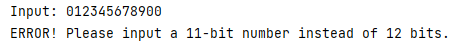
\includegraphics[width=1\linewidth]{../pic/1/1.6.png}
	\end{subfigure}
    \vspace{1cm}
    \begin{subfigure}{0.325\linewidth}
		\centering
		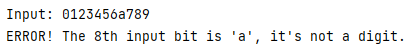
\includegraphics[width=1\linewidth]{../pic/1/1.7.png}
	\end{subfigure}
	\begin{subfigure}{0.325\linewidth}
		\centering
		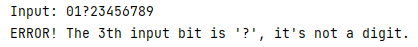
\includegraphics[width=1\linewidth]{../pic/1/1.8.png}
	\end{subfigure}
	\begin{subfigure}{0.325\linewidth}
		\centering
		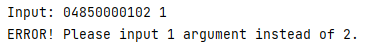
\includegraphics[width=1\linewidth]{../pic/1/1.9.png}
	\end{subfigure}
	\caption{Output of Problem1}
\end{figure}

\newpage
\section{实验2. 数字转英语}

    \lstinputlisting[
        language = Java, 
        caption = {\bf Problem2.java}
    ]{../../../ProblemSet/src/Problem2.java}

    \begin{figure}[H]
        \centering
        \begin{subfigure}{0.13\linewidth}
            \centering
            
\includegraphics[width=0.5\linewidth]{../pic/2/2.1.png}
            \caption{input: 0}
        \end{subfigure}
        \begin{subfigure}{0.17\linewidth}
            \centering
            
\includegraphics[width=1\linewidth]{../pic/2/2.2.png}
            \caption{input: -1}
        \end{subfigure}
        \begin{subfigure}{0.17\linewidth}
            \centering
            
\includegraphics[width=1\linewidth]{../pic/2/2.3.png}
            \caption{input: 100}
        \end{subfigure}
        \begin{subfigure}{0.17\linewidth}
            \centering
            
\includegraphics[width = 1\linewidth]{../pic/2/2.4.png}
            \caption{input: 1000}
        \end{subfigure}
        \begin{subfigure}{0.27\linewidth}
            \centering
            
\includegraphics[width=1\linewidth]{../pic/2/2.5.png}
            \caption{input: 5000210}
        \end{subfigure}
        \begin{subfigure}{1\linewidth}
            \centering
            
\includegraphics[width=0.9\linewidth]{../pic/2/2.6.png}
            \caption{input: 999999999}
        \end{subfigure}
        \caption{Output of Problem2}
    \end{figure}

\newpage
\section{实验3. 长度n的子序列最大乘积}
    \lstinputlisting[
            language = Java, 
            caption = {\bf Problem3.java}
    ]{../../../ProblemSet/src/Problem3.java}
    \begin{figure}[H]
        \centering
        
\includegraphics[width = 0.4\textwidth]{../pic/3/3.1.png}
        \caption{Output of Problem3}
    \end{figure}

\newpage
\section{实验4. 模式化打印图形}
    \lstinputlisting[
            language = Java, 
            caption = {\bf Problem4.java}
    ]{../../../ProblemSet/src/Problem4.java}
    \begin{figure}[H]
        \centering
        \begin{subfigure}{0.19\linewidth}
            \centering
            
\includegraphics[width=1\linewidth]{../pic/4/4.a.png}
            \caption{input: a 7}
        \end{subfigure}
        \begin{subfigure}{0.19\linewidth}
            \centering
            
\includegraphics[width=1\linewidth]{../pic/4/4.b.png}
            \caption{input: b 7}
        \end{subfigure}
        \begin{subfigure}{0.19\linewidth}
            \centering
            
\includegraphics[width=1\linewidth]{../pic/4/4.c.png}
            \caption{input: c 7}
        \end{subfigure}
        \begin{subfigure}{0.19\linewidth}
            \centering
            
\includegraphics[width = 1\linewidth]{../pic/4/4.d.png}
            \caption{input: d 7}
        \end{subfigure}
        \begin{subfigure}{0.19\linewidth}
            \centering
            
\includegraphics[width=1\linewidth]{../pic/4/4.e.png}
            \caption{input: e 7}
        \end{subfigure}
        \caption{Output of Problem4}
    \end{figure}

\newpage
\section{实验5. 直方统计图}
\lstinputlisting[
    language = Java, 
    caption = {\bf Problem5.java}
]{../../../ProblemSet/src/Problem5.java}
\begin{figure}[H]
    \centering
    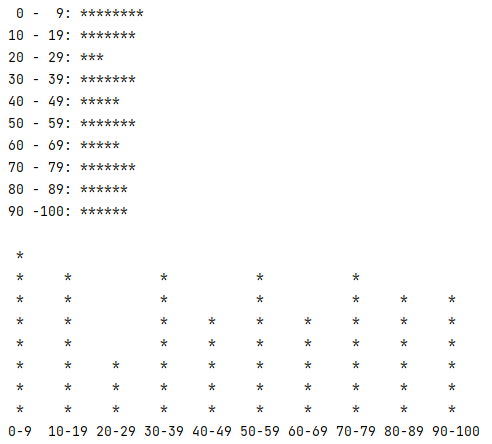
\includegraphics[width = 0.5\textwidth]{../pic/5/5.1.png}
    \caption{Output of Problem5}
\end{figure}

\newpage
\section{实验6. 直方统计图}
\lstinputlisting[
    language = Java, 
    caption = {\bf Problem6.java}
]{../../../ProblemSet/src/Problem6.java}
\begin{figure}[H]
    \centering
    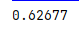
\includegraphics[width = 0.15\textwidth]{../pic/6/6.1.png}   
    \caption{Output of Problem6} 
\end{figure}
    
